\documentclass[preview, 11pt]{standalone}
% The next four lines ensure reproducible builds
% https://tex.stackexchange.com/q/229605
\pdfinfoomitdate=1
\pdftrailerid{}
\pdfsuppressptexinfo=1
\pdfinfo{ /Creator () /Producer () }
\newcommand{\ident}[1]{\textnormal{#1}}
\usepackage{amsmath}
\DeclareMathOperator{\best}{best}
\DeclareMathOperator{\choices}{choices}
\def\Din{X}
\def\Dout{Y}
\def\D{\textnormal{\color{red} REPLACE ME WITH Din OR Dout}}
\usepackage[dvipsnames]{xcolor}
\usepackage{tikz}
\usetikzlibrary{positioning}
\usetikzlibrary{shapes.geometric}
\usetikzlibrary{arrows.meta}
\begin{document}
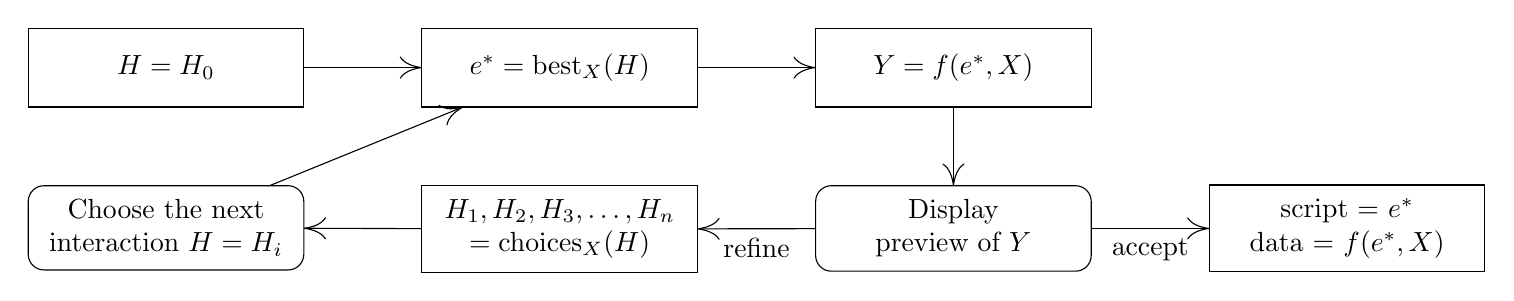
\begin{tikzpicture}[%
	base/.style={draw=black, align=center, outer sep=0pt, minimum
		width=35mm, minimum height=10mm, inner sep=5pt},
	rect/.style={base},
	rounded/.style={base, rounded corners=2mm},%
	arrow/.style={arrows={->[scale=4, length=2, width=2]}}%
	]
	%
	% Nodes
	%
	\node[rect] (ENTER) at (0, 0) {$H = H_0$};
	\node[rect, right=1.5cm of ENTER] (BEST) {$e^* = \best_\Din(H)$};
	\node[rect, right=1.5cm of BEST] (RESULT) {$\Dout = f(e^*, \Din)$};
	\node[rounded, below=1cm of RESULT] (PREVIEW) {Display\\ preview of $\Dout$};
	\node[rect, right=1.5cm of PREVIEW] (OUT) {script = $e^*$ \\ data = $f(e^*, \Din)$};
	\node[rect, below=1cm of BEST] (CHOICES) {$H_1, H_2, H_3, \ldots, H_n$\\ $= \choices_\Din(H)$};
	\node[rounded, below=1cm of ENTER] (INTERACT) {Choose the next \\ interaction $H = H_i$};
	\path[arrow] (BEST) edge (RESULT);
	\path[arrow] (INTERACT) edge (BEST);
	\path[arrow] (RESULT) edge (PREVIEW);
	\path[arrow] (PREVIEW) edge node[midway, below] {accept} (OUT);
	\path[arrow] (PREVIEW) edge node[midway, below] {refine} (CHOICES);
	\path[arrow] (CHOICES) edge (INTERACT);
	\path[arrow] (ENTER) edge (BEST);
\end{tikzpicture}
\end{document}
